% WebContactsProPlus — sequence: POST /api/v1/contacts
\documentclass[border=14pt]{standalone}
\usepackage{tikz}
\usetikzlibrary{positioning, arrows.meta, calc, fit}

\begin{document}
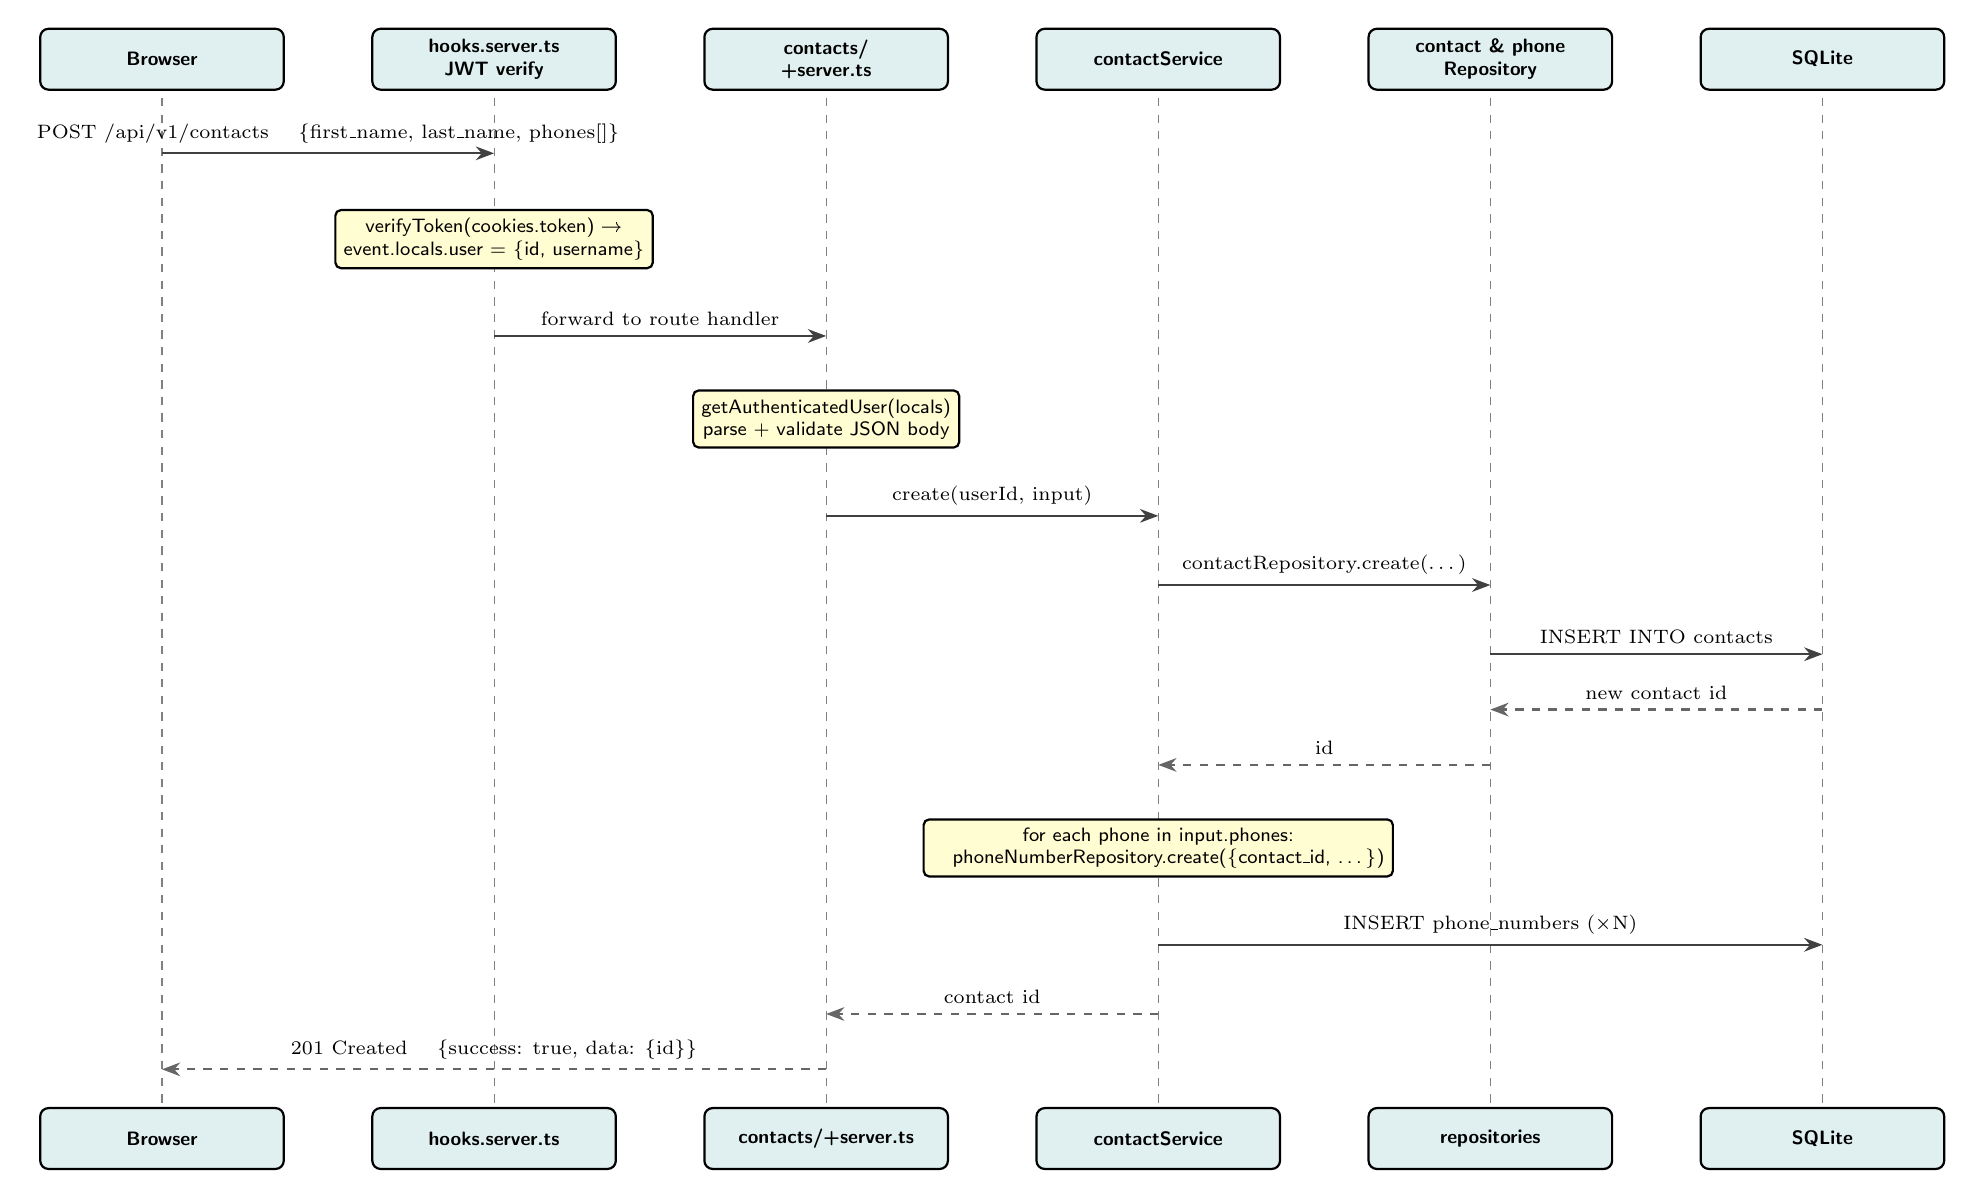
\begin{tikzpicture}[
    >=Stealth,
    font=\sffamily\footnotesize,
    actor/.style={
        draw, thick, fill=teal!12, rounded corners=3pt,
        minimum width=88pt, minimum height=22pt,
        align=center, font=\sffamily\scriptsize\bfseries,
    },
    msg/.style={->, thick, draw=black!75},
    ret/.style={->, thick, draw=black!60, dashed},
    note/.style={
        draw, thick, fill=yellow!18,
        rounded corners=2pt, align=center,
        font=\sffamily\scriptsize, inner sep=3pt,
    },
    lifeline/.style={dashed, draw=black!50},
]

\def\colA{0}
\def\colB{120}
\def\colC{240}
\def\colD{360}
\def\colE{480}
\def\colF{600}

\node[actor] (A) at (\colA pt,0) {Browser};
\node[actor] (B) at (\colB pt,0) {hooks.server.ts \\ {\scriptsize JWT verify}};
\node[actor] (C) at (\colC pt,0) {contacts/\\+server.ts};
\node[actor] (D) at (\colD pt,0) {contactService};
\node[actor] (E) at (\colE pt,0) {contact \& phone\\Repository};
\node[actor] (F) at (\colF pt,0) {SQLite};

\def\bot{-390pt}
\foreach \x in {\colA, \colB, \colC, \colD, \colE, \colF}
    \draw[lifeline] (\x pt,-14pt) -- (\x pt,\bot);

\node[actor] at (\colA pt, \bot) {Browser};
\node[actor] at (\colB pt, \bot) {hooks.server.ts};
\node[actor] at (\colC pt, \bot) {contacts/+server.ts};
\node[actor] at (\colD pt, \bot) {contactService};
\node[actor] at (\colE pt, \bot) {repositories};
\node[actor] at (\colF pt, \bot) {SQLite};

% messages
\draw[msg] (\colA pt,-34pt) -- node[above, font=\scriptsize] {POST /api/v1/contacts \quad \{first\_name, last\_name, phones[]\}} (\colB pt,-34pt);

\node[note] (n1) at (\colB pt,-65pt) {
    verifyToken(cookies.token) → \\
    event.locals.user = \{id, username\}
};

\draw[msg] (\colB pt,-100pt) -- node[above, font=\scriptsize] {forward to route handler} (\colC pt,-100pt);

\node[note] (n2) at (\colC pt,-130pt) {
    getAuthenticatedUser(locals) \\
    parse + validate JSON body
};

\draw[msg] (\colC pt,-165pt) -- node[above, font=\scriptsize] {create(userId, input)} (\colD pt,-165pt);
\draw[msg] (\colD pt,-190pt) -- node[above, font=\scriptsize] {contactRepository.create(\dots)} (\colE pt,-190pt);
\draw[msg] (\colE pt,-215pt) -- node[above, font=\scriptsize] {INSERT INTO contacts} (\colF pt,-215pt);
\draw[ret] (\colF pt,-235pt) -- node[above, font=\scriptsize] {new contact id} (\colE pt,-235pt);
\draw[ret] (\colE pt,-255pt) -- node[above, font=\scriptsize] {id} (\colD pt,-255pt);

\node[note] (n3) at (\colD pt,-285pt) {
    for each phone in input.phones: \\
    \quad phoneNumberRepository.create(\{contact\_id, \dots\})
};

\draw[msg] (\colD pt,-320pt) -- node[above, font=\scriptsize] {INSERT phone\_numbers (×N)} (\colF pt,-320pt);

\draw[ret] (\colD pt,-345pt) -- node[above, font=\scriptsize] {contact id} (\colC pt,-345pt);
\draw[ret] (\colC pt,-365pt) -- node[above, font=\scriptsize] {201 Created \quad \{success: true, data: \{id\}\}} (\colA pt,-365pt);

\end{tikzpicture}
\end{document}
